\chapter{Background Information on Binary Decision Diagrams}

\textit{This chapter provides background information on Binary Decision Diagrams.}

\section{Preliminaries}
A Binary Decision Diagram is a data structure used to efficiently represent boolean functions. BDDs were introduced by \cite{akers1978binary} in 1978 to compress large digital (boolean) functions. BDDs were further developed by Bryant \cite{bryant1986graph, bryant1992symbolic} in 1986 and 1992. The following definition is taken from \cite{sylvan_multicore_bdd}:

\begin{definition}
	An (ordered) Binary Decision Diagram (BDD) is a directed acyclic graph with the following properties:
	\begin{enumerate}
		\item There is a single root node and two terminal nodes $0$ and $1$.
		\item Each non-terminal node $p$ has a variable $var(p) = x_i$ and two outgoing edges, labeled $0$ and $1$; we write $lvl(p) = i$ and $p[v] = q$, where $v \in \{ 0, 1 \}$
		\item For each edge from node $p$ to non-terminal node $q$, $lvl(p) < lvl(q)$.
		\item There are no duplicate nodes, i.e. $\forall p \forall q .(lvl(p) = lvl(q) \wedge p[0] = q[0] \wedge p[1] = q[1]) \implies p = q$
	\end{enumerate}
\end{definition}

In Figure \ref{fig:bdd_examples} four different simple boolean functions are represented as a BDD. The rectangle-shaped nodes are the terminal nodes $0$ and $1$ and all other nodes represent a variable. Every non-terminal node $p$ has two edges, namely a thick one representing $p[1]$ and a dashed one representing $p[0]$. All paths in the BDD that lead to the terminal node $1$ makes the boolean function represented by the BDD to evaluate to true.

\begin{figure}
	\centering
	\subfloat[$x$] {
		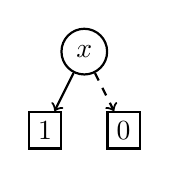
\begin{tikzpicture}
\node[circle, thick, draw] (v1) at (0,1) {$x$};
\node[rectangle, thick, draw] (v2) at (-0.5,0) {$1$};
\node[rectangle, thick, draw] (v3) at (0.5,0) {$0$};

\draw[->, thick]  (v1) edge (v2);
\draw[->, thick, dashed]  (v1) edge (v3);

\end{tikzpicture}
		$\vspace{360pt}$
	}
	$\hspace{36pt}$
	\subfloat[$\neg x$] {
		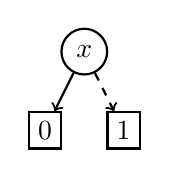
\begin{tikzpicture}
\node[circle, thick, draw] (v1) at (0,1) {$x$};
\node[rectangle, thick, draw] (v2) at (-0.5,0) {$0$};
\node[rectangle, thick, draw] (v3) at (0.5,0) {$1$};

\draw[->, thick]  (v1) edge (v2);
\draw[->, thick, dashed]  (v1) edge (v3);

\end{tikzpicture}
	}
	$\hspace{36pt}$
	\subfloat[$x_0 \wedge x_1$] {
		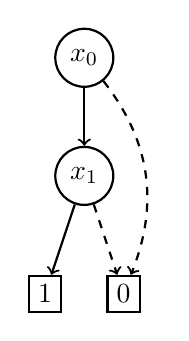
\begin{tikzpicture}
\node[circle, thick, draw] (v4) at (0,3) {$x_0$};
\node[circle, thick, draw] (v1) at (0,1.5) {$x_1$};
\node[rectangle, thick, draw] (v2) at (-0.5,0) {$1$};
\node[rectangle, thick, draw] (v3) at (0.5,0) {$0$};

\draw[->, thick]  (v1) edge (v2);
\draw[->, thick, dashed]  (v1) edge (v3);

\draw[->, thick]  (v4) edge (v1);
\draw[->, thick, dashed]  (v4) edge [bend left=30 ] (v3);

\end{tikzpicture}
	}
	$\hspace{36pt}$
	\subfloat[$x_0 \vee x_1$] {
		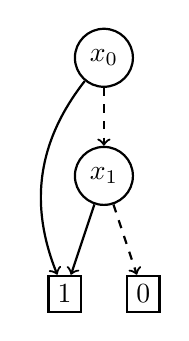
\begin{tikzpicture}
\node[circle, thick, draw] (v4) at (0,3) {$x_0$};
\node[circle, thick, draw] (v1) at (0,1.5) {$x_1$};
\node[rectangle, thick, draw] (v2) at (-0.5,0) {$1$};
\node[rectangle, thick, draw] (v3) at (0.5,0) {$0$};

\draw[->, thick]  (v1) edge (v2);
\draw[->, thick, dashed]  (v1) edge (v3);

\draw[->, thick]  (v4) edge [bend right=30 ] (v2);
\draw[->, thick, dashed]  (v4) edge (v1);

\end{tikzpicture}
	}
	
	\caption{The BDD representation of four different simple boolean functions are displayed.}
	\label{fig:bdd_examples}
\end{figure}

It is possible to represent a set of states $S \subseteq U$ from some universe $U$ by a boolean function $f : S \rightarrow \mathbb{B}$, such that $S = \{ x \in U \ | \ f(x) \}$. If $U = \mathbb{B}^n$, then $f$ is a function with signature $f : \mathbb{B}^n \rightarrow \mathbb{B}$ and so $f$ can be represented as a BDD. 

By applying this trick the state space of some program can efficiently be represented as a BDD. Suppose that the program uses a set of variable names $X = \{ x_1, \dots, x_n \}$ and we have an assignment function $v : X \rightarrow \mathbb{B}$. Then $U = \mathbb{B}^n$ can represent all possible variable assignments under $v$ and $S = \mathbb{B}^n$ represents all reachable states. Now a boolean function $f : S = \mathbb{B}^n \rightarrow \mathbb{B}$ can be given. Suppose that the program uses a transition relation $R \subseteq S \times S$. Then the same trick can be applied again to represent $R$.

We now introduce reduced ordened BDDs.

\begin{definition}
	A \emph{Reduced Ordened BDD (ROBDD)} is an ordened BDD without redundant nodes. A node $p$ is redundent if $p[0] = p[1]$.
\end{definition}

\begin{figure}
	\centering
	\subfloat[BDD with duplicate nodes] {
		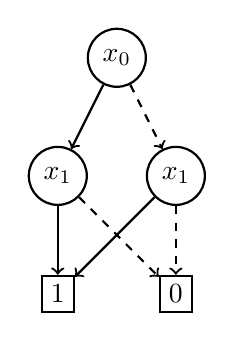
\begin{tikzpicture}
\node[circle, thick, draw] (v4) at (0.25,3) {$x_0$};
\node[circle, thick, draw] (v1) at (-0.5,1.5) {$x_1$};
\node[circle, thick, draw] (v5) at (1,1.5) {$x_1$};
\node[rectangle, thick, draw] (v2) at (-0.5,0) {$1$};
\node[rectangle, thick, draw] (v3) at (1,0) {$0$};

\draw[->, thick]  (v1) edge (v2);
\draw[->, thick, dashed]  (v1) edge (v3);
\draw[->, thick]  (v4) edge (v1);
\draw[->, thick, dashed]  (v4) edge (v5);
\draw[->, thick]  (v5) edge (v2);
\draw[->, thick, dashed]  (v5) edge (v3);

\end{tikzpicture}
		$\vspace{360pt}$
	}
	$\hspace{36pt}$
	\subfloat[BDD with a redundant node] {
		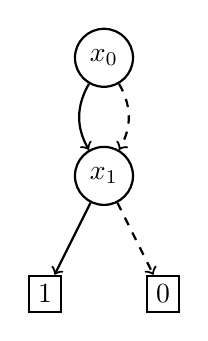
\begin{tikzpicture}
\node[circle, thick, draw] (v4) at (0.25,3) {$x_0$};
\node[circle, thick, draw] (v1) at (0.25,1.5) {$x_1$};

\node[rectangle, thick, draw] (v2) at (-0.5,0) {$1$};
\node[rectangle, thick, draw] (v3) at (1,0) {$0$};

\draw[->, thick]  (v1) edge (v2);
\draw[->, thick, dashed]  (v1) edge (v3);
\draw[->, thick]  (v4) edge [bend right=30] (v1);
\draw[->, thick, dashed]  (v4) edge [bend left=30] (v1);


\end{tikzpicture}
	}
	$\hspace{36pt}$
	\subfloat[Reduced Ordened BDD] {
		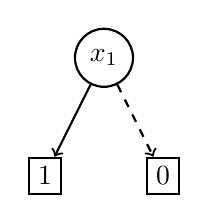
\begin{tikzpicture}

\node[circle, thick, draw] (v1) at (0.25,1.5) {$x_1$};

\node[rectangle, thick, draw] (v2) at (-0.5,0) {$1$};
\node[rectangle, thick, draw] (v3) at (1,0) {$0$};

\draw[->, thick]  (v1) edge (v2);
\draw[->, thick, dashed]  (v1) edge (v3);



\end{tikzpicture}
	}
	
	\caption{Three BDD representations of the boolean function $(x_0 \wedge x_1) \vee (\overline{x_0} \wedge x_1)$ (left representation), which is equivalent to $x_1$ (right representation). The rightmost BDD is obtained by removing duplicates and redundant nodes.}
	\label{fig:bdd_reductions}
\end{figure}

Figure \ref{fig:bdd_reductions} shows examples of BDDs that have duplicate nodes an redundant nodes. In Figure \ref{fig:bdd_reductions} all three BDDs are equivalent to each other, only the rightmost one is reduced and ordened. 

\section{Sequential BDD operations}
BDD operations use two tables, namely a \emph{Unique Table} and a \emph{Computed Table}. The unique table is used to store BDD nodes and is necessary to ensure that there are no duplicate nodes. The unique table is usually implemented as a hash table. The computed table acts as a cache. Most of the BDD operations are recursively defined, and the subresults are stored in the computed table. Before performing recursive calls the operations can check if the operation has been done before.

Most BDD operations are based on a concept called Shannon decomposition \cite{dijk2012parallelization}, which is defined below.

\begin{definition}[Restriction]
	Let $X = \{ x_1, \dots, x_n \}$ be a set of variable names and $\phi(x_1, \dots, x_n)$ a boolean formula (i.e. with codomain $\mathbb{B}$). Then the \emph{restriction} of $v$ to $x_i \in X$ in $\phi$, denoted by $\phi_{x_i=v}$, is defined by 
	\begin{equation}
		\phi_{x_i=v} \equiv \phi(x_1, \dots, x_{i - 1}, v, x_{i + 1}, \dots, x_n)
	\end{equation}
\end{definition}

\begin{definition}[Shannon Decomposition]
	Let $X = \{ x_1, \dots, x_n \}$ be a set of variable names and $\phi(x_1, \dots, x_n)$ a boolean formula (i.e. with codomain $\mathbb{B}$). Then the \emph{Shannon decomposition} of $\phi$ along $x \in X$ is defined as $\psi = (x \wedge \phi_{x=1}) \vee (\overline{x} \wedge \phi_{x=0})$ such that $\phi \equiv \psi$. 
\end{definition}

Many BDD operations are implemented by taking some variable $x$ and recursively calculating the results of the subproblems $\phi_{x=0}$ and $\phi_{x=1}$ by making a BDD of the Shannon decomposition of $\phi$ along $x$. 

Furthermore existential quantification and substitution is needed to implement the \emph{relational product} operation.

\begin{definition}[Existential Quantification]
	Let $X = \{ x_1, \dots, x_n \}$ be a set of variable names and $\phi$ be a boolean function. Take $x \in X$. Then existential quantification is defined as $\exists x \phi = \phi_{x=0} \vee \phi_{x=1}$. Take $X' = \{ x'_1, \dots, x'_m \} \subseteq X$. Then $\exists X' \phi \equiv \exists x'_1, \dots, \exists x'_m \phi$.
\end{definition}

\begin{definition}[Substitution]
	Let $X = \{ x_1, \dots, x_n \}$ be a set of variable names and $\phi$ be a boolean function. Take $x_i, y \in X$. Then substitution is defined by:
	\begin{equation}
		\phi[x_i \gets y] \equiv \phi(x_1, \dots, x_{i - 1}, y, x_{i + 1}, \dots, x_n)
	\end{equation}
	Now consider two sets $Y = \{ y_1, \dots, y_m \} \subseteq X$ and $Z = \{ z_1, \dots, z_m \} \subseteq X$ of variable names. Then $\phi[Y \gets Z]$ is defined as:
	\begin{equation}
		\phi[Y \gets Z] \equiv (((\phi[y_1 \gets z_1])[y_2 \gets z_2]) \dots [y_m \gets z_m])
	\end{equation}
\end{definition}

The following two sections describe the two basic BDD operations \texttt{ite} and \texttt{relprod}.

\subsection{The \texttt{ite} operation}
Many BDD operations can be expressed with the \texttt{ite} operation (which stands for if-then-else). This operation is specified as \cite{dijk2012parallelization}:
\begin{equation}
	\texttt{ite}(A, B, C) \equiv (A \wedge B) \vee (\overline A \wedge C)
\end{equation}
where $A, B, C$ are boolean formulas. Table \ref{tab:ite} shows a number of boolean formulas expressed with the \texttt{ite} operation.

\begin{table}[ht]
	\centering
	\begin{tabular}{| c | l |}
		\hline
		Operator & ITE \\ 
		\hline 
		$F \wedge G$ & $\texttt{ite}(F, G, 0)$ \\
		$F \vee G$ & $\texttt{ite}(F, 1, G)$ \\
		$F \oplus G$ & $\texttt{ite}(F, \overline G, G)$ \\
		$\neg (F \wedge G)$ & $\texttt{ite}(F, \overline G, 1)$ \\
		$\neg (F \vee G)$ & $\texttt{ite}(F, 0, \overline G)$ \\
		$F \rightarrow G$ & $\texttt{ite}(F, G, 1)$ \\
		$F \leftarrow G$ & $\texttt{ite}(F, 1, \overline G)$ \\
		$F \leftrightarrow G$ & $\texttt{ite}(F, G, \overline G)$ \\
		$\overline F \wedge G$ & $\texttt{ite}(F, 0, G)$ \\
		$F \wedge \overline G$ & $\texttt{ite}(F, \overline G, 0)$ \\
		\hline
	\end{tabular}
	\caption{This table shows several boolean formulas expressed with the \texttt{ite} operation. This table is taken from \cite{dijk2012parallelization}.}
	\label{tab:ite}
\end{table}

\begin{figure}
	\centering
	\begin{algorithm}[H]
		\SetStartEndCondition{ }{}{}%
		\SetKwProg{Fn}{bdd}{\string:}{}
		\SetKwFunction{fun}{ite}
		\SetKw{KwTo}{in}\SetKwFor{For}{for}{\string:}{}%
		\SetKwIF{If}{ElseIf}{Else}{if}{}{elif}{else}{}%
		\SetKwFor{While}{while}{:}{fintq}%
		\SetKw{test}{in}{}%
		\AlgoDontDisplayBlockMarkers\SetAlgoNoEnd\SetAlgoNoLine%

		\Fn{\fun{\textbf{bdd} $A$, \textbf{bdd} $B$, \textbf{bdd} $C$}} {
			\textbf{if} $A=1$ \textbf{return} $B$ \\
			\textbf{if} $A=0$ \textbf{return} $C$ \\
			\textbf{if} $\texttt{in-cache}(A, B, C)$ \textbf{return} $\texttt{cache-lookup}(A,B,C)$ \\
			$x \gets \texttt{min}(\texttt{var}(A), \texttt{var}(B), \texttt{var}(C))$ \\
			$R_{low} \gets \texttt{ite}(\texttt{low}(A, x), \texttt{low}(B, x), \texttt{low}(C, x))$ \\
			$R_{high} \gets \texttt{ite}(\texttt{high}(A, x), \texttt{high}(B, x), \texttt{high}(C, x))$ \\
			$R \gets \texttt{mk}(x, R_{low}, R_{high})$ \\
			$\texttt{add-to-cache}(A, B, C, R)$ \\
			\Return{$R$}
		}
	\end{algorithm}

	\caption{The (sequential) implementation of the \texttt{ite} operation.}
	\label{fig:ite_seq}
\end{figure}

The implementation of the \texttt{ite} function is given in Figure \ref{fig:ite_seq}. Instead of taking three boolean formulas, the implementation takes their BDD representations. The \texttt{in-cache}, \texttt{cache-lookup}, and \texttt{add-to-cache} functions tests if the BDD is in the computed table, gets the BDD from the computed table and adds the BDD to the computed table, respectively.

The operations \texttt{low} and \texttt{high} calculate the \emph{cofactor} of their first operand. These two functions are specified as follows:
\begin{equation}
	\texttt{low}(F, x) \equiv F_{x=0}
\end{equation}
\begin{equation}
	\texttt{high}(F, x) \equiv F_{x=1}
\end{equation}

The \texttt{mk} function creates a new BDD node and adds it to the unique table.

\subsection{The \texttt{relprod} operation}
Binary Decision Diagrams are used in symbolic model checking. An important model checking algorithm is the \emph{reachability} algorithm, which determines the set of all reachable program states, given an initial state and a transition relation. 

Burch et al. \cite{burch1994symbolic} used the \emph{relational product} operation to implement the reachability algorithm, where both the initial state and the transition relation function are represented by boolean functions. The relational product has the form $\exists X. (A \wedge B)$, where $X$ is a set of variables and $A, B$ are boolean functions.

Let $X = \{ x_1, \dots, x_n \}$ be a set of variable names. Suppose that $\phi(x_1, \dots, x_n) \equiv \phi(X)$ represent a set of states and $\psi(x_1, \dots, x_n, x'_1, \dots, x'_n) \equiv \psi(X, X')$ represent the transition relation. Then \texttt{relprod} is used to calculate the next set of states $\phi'(X)$ by:
\begin{equation}
	\phi'(X') \equiv \exists X. (\phi(X) \wedge \psi(X, X'))
	\label{eqn:relprod_1}
\end{equation}
\begin{equation}
	\phi'(X) \equiv \phi'(X')[X' \gets X]
	\label{eqn:relprod_2}
\end{equation}
Note that $\phi(X)$ is used in \ref{eqn:relprod_1} so that the successors calculated by $\psi(X, X')$ are limited to states represented by $\phi(X)$. Then all variable names of $X$ are abstracted, so that only variable names in $X'$ remain. The last step, which is performed in \ref{eqn:relprod_2}, is to rename all variable names from $X'$ to $X$. This is done by applying substitution. The result is the set of states $\phi'(X)$ reachable from $\phi(X)$ by applying the transition relation.

\begin{figure}
	\centering
	\begin{algorithm}[H]
		\SetStartEndCondition{ }{}{}%
		\SetKwProg{Fn}{bdd}{\string:}{}
		\SetKwFunction{fun}{relprod}
		\SetKw{KwTo}{in}\SetKwFor{For}{for}{\string:}{}%
		\SetKwIF{If}{ElseIf}{Else}{if}{}{elif}{else}{}%
		\SetKwFor{While}{while}{:}{fintq}%
		\SetKw{test}{in}{}%
		\AlgoDontDisplayBlockMarkers\SetAlgoNoEnd\SetAlgoNoLine%

		\Fn{\fun{\textbf{bdd} $A$, \textbf{bdd} $B$, $X$}} {
			\textbf{if} $A=1 \wedge B=1$ \textbf{return} $1$ \\
			\textbf{if} $A=0 \vee B=0$ \textbf{return} $0$ \\
			\textbf{if} $\texttt{in-cache}(A, B, X)$ \textbf{return} $\texttt{cache-lookup}(A, B, X)$ \\
			$x \gets \texttt{min}(\texttt{var}(A), \texttt{var}(B))$ \\
			$R_{low} \gets \texttt{relprod}(\texttt{low}(A, x), \texttt{low}(B, x), X)$ \\
			$R_{high} \gets \texttt{relprod}(\texttt{high}(A, x), \texttt{high}(B, x), X)$ \\

			\If{$x \in X$} {
				$R \gets \texttt{ite}(R_{low}, 1, R_{high})$
			}
			\Else {
				$R \gets \texttt{mk}(x, R_{low}, R_{high})$ \\
			}
			
			$\texttt{add-to-cache}(A, B, X, R)$ \\
			\Return{$R$}
		}
	\end{algorithm}

	\caption{The (sequential) implementation of the \texttt{relprod} operation.}
	\label{fig:relprod_seq}
\end{figure}

Figure \ref{fig:relprod_seq} shows an implementation of the \texttt{relprod} function. The implementation of \cite{dijk2012parallelization} shows that if $x \in X$ and $R_{low} = 1$ then the result $1$ can simply be returned. This algorithm however shows the essence of the relational product implementation. \cite{dijk2012parallelization} also gives a new algorithm \texttt{relprods} that is more efficient than \texttt{relprod} because it does not create BDD nodes unnecessarily.

\section{Garbage Collection}
Unfinished..

\section{Parallel BDD operations}
A parallel version of the \texttt{ite} and \texttt{relprod} operations is given in \cite{dijk2012parallelization} and \cite{sylvan_multicore_bdd}. The unique table and the computed table are implemented using the lockless hash table described in \cite{so73119}. Furthermore the recursive calls in Figures \ref{fig:ite_seq} and \ref{fig:relprod_seq} are done in parallel by using a work stealing framework. The implementation of \cite{dijk2012parallelization} uses the Wool framework \cite{faxen2010efficient} and the implementation of \cite{sylvan_multicore_bdd} uses Lace \cite{dijk2013lace}.